\documentclass{article}
\usepackage{graphicx} % Required for inserting images

% Language setting
% Replace `english' with e.g. `spanish' to change the document language
\usepackage[english]{babel}

% Set page size and margins
% Replace `letterpaper' with`a4paper' for UK/EU standard size
\usepackage[letterpaper,top=2cm,bottom=2cm,left=3cm,right=3cm,marginparwidth=1.75cm]{geometry}

% Useful packages
\usepackage{xcolor}
\usepackage{amssymb}
\usepackage{amsmath}
\usepackage{graphicx}
\usepackage[colorlinks=true, allcolors=blue]{hyperref}
\usepackage{cleveref}


\newcommand{\studentName}{Nicolas RECHATIN-NOËL}
\newcommand{\internshipTopic}{my internship topic}
\newcommand{\internshipWeeks}{12}

\newcommand{\phaseOne}{A exhaustive collection of articles related to \internshipTopic}
\newcommand{\phaseTwo}{Implementing complex science}
\newcommand{\phaseThree}{Developing new complex science}
\newcommand{\phaseFour}{Mathematical proofs that my devlopments work}
\newcommand{\phaseFive}{Conculsion on my intership}
\newcommand{\phaseSix}{Final Report}

\title{Early work on ``Adaptive polyhedral mesh refinement for numerical simulation''}
\author{\studentName}

\begin{document}
\maketitle

\section{Introduction}
Meshing is a crucial part of all numerical simulations. Thus, exploring new meshing technologies and the ecosystem of tools around them has been, and will always be, a field of research aimed at increasing numerical simulation possibilities—whether in terms of accuracy, performance, or robustness of the solutions. Over time, as the number of methods increases, selecting the appropriate mesh to match the simulated physics and the chosen method is becoming increasingly challenging. That said, exploring different types of meshing techniques and how to optimize simulations with them across various methods can significantly enhance results if the appropriate physics are adapted. As poly meshes have gained traction in the community in recent years, we aimed to explore where the current state of the art stands. Which fields of physics benefit the most from this technology? What are the primary benefits attributed to polygonal meshes in those cases, and are there others to explore? Are there any tools missing in the polygonal meshing ``ecosystem'' that could lead to further improvements?

In this thesis, we believe that exploring new approaches and improving existing ones for adaptive mesh refinement with these types of meshes could be a valuable addition to numerical simulations. Before delving into that, we decided to solidify our understanding of what polyhedral meshes can contribute to simulations. To achieve this, we benchmarked several simple polygonal meshes against other quadratic or triangular meshes to observe how, and in which cases, polygonal meshes could yield better results through basic refinements. Finally, to expand on these preliminary results, we sought to examine the directions in which the community is moving, particularly in terms of which fields of physics and methods seem to benefit the most from these meshes.

With all this in mind, these first few months of work were dedicated to achieving three main goals:
\begin{enumerate}
\item Becoming familiar with the ``world'' of meshing—its methods, vocabulary, tools, and optimizations—primarily through reading and experimentation.
\item Understanding the particularities and challenges that polygonal and polyhedral meshes present by reviewing the current state of the art and the challenges faced by the community.
\item Making an informed decision on how we intend to simulate polygonal and polyhedral meshes for adaptive mesh refinement. This involves choosing the mesh type and mesher, the method, and the physics we will simulate, based on what we believe will provide the best robustness or optimization.
\end{enumerate}

\section{Experimenting on polygonal and polyhedral meshes}

\subsection{Current interest for polyhedral meshing simulation.}
Formulations for several finite element method does exist for polyhedral elements since years has seen in~\cite{rashid2006three,bishop2014displacement,gain2014virtual}. However, as cited in~\cite{bishop2020polyhedral} ``despite recent research in the development of polyhedral finite element formulations, the development of general purpose polyhedral meshing tools is lacking''.

Over the past ten years, there has been a growing body of publications focused on demonstrating and enhancing the capabilities of polygonal and polyhedral meshes. Early works, such as~\cite{spiegel2011tetrahedral}, compared tetrahedral and polyhedral meshes, while more recent studies~\cite{vacca2017virtual,lipnikov2011mimetic,antonietti2018high} started studying new methods tailored to polyhedral meshes across various physics domains. Additionally, much more recent research has begun to explore how new technologies can enhance polyhedral meshing simulations~\cite{antonietti2022machine} or apply it to recent challenges~\cite{LI2024111846}. This body of work reflects the significant development of polygonal and polyhedral meshes in numerical simulation, evolving from merely being evaluated to being optimized and built upon.

Among many different kinds of meshes which can be chosen for performing a numerical simulation, this new class of meshes – polyhedral meshes – is gaining in popularity. Recently, many numerical methods such as finite-elements and finite-volumes have started to adopt polyhedral discretization. Rightly so, as these meshes/discretization bring along advantages such as lower space complexity during meshing, lower CPU memory costs, higher-accuracy for solution, etc. Despite these recent advances in polyhedral discretization, a general purpose algorithm (mesher) that provides such meshes in a robust manner is lacking. Via this work, we intend to explore the subject of polyhedral meshing and re-meshing. Globally, the aim will be two-folds. First study/analyze/develop a polyhedral meshing algorithm/mesher. Second, for solution-accuracy and the computational cost associated to polyhedral discretization provide means for mesh adaption.

We now have a lot more studies made regarding those numerical methods used for polyhedral meshes. Methods like Discontinuous Galerkin~\cite{dong2018discontinuous,antonietti2021high}, Mimetic Finite Difference~\cite{da2009mimetic,lipnikov2011mimetic,da2014mimetic}, Virtual Element Method~\cite{cangiani2017virtual,sorgente2022polyhedral} and other one have mature other the years on the subject. So we believe that addressing the development of polyhedral meshing tools could benefit from all this research regarding numerical methods.


\subsection{Early benchmark for polytopal meshes}

Although this work was primarily for learning purposes, focusing on the first two objectives outlined earlier, we also aimed to create a preliminary benchmark for the tools we intend to rely on in the coming months. Developing such a benchmark requires a comprehensive understanding of the entire process—from geometry generation to simulation results, post-processing, and evaluation—while also becoming familiar with the tools involved at each stage.

\subsubsection{Goals}
Building on previous work conducted in our lab at CEA, as detailed in~\cite{nora2022dualPoly}, we aimed to replicate part of the study to validate our expectations regarding the behavior of polygonal and polyhedral simulations across multiple refinements. The objective here was not to adjust the mesh to the simulation, but rather to observe how the model converges using polygonal meshes generated via the ``smooth-dual'' approach while adding more cells. Since we are employing a method called ``PolyMac'' which is currently under research at CEA, our initial step was to verify its convergence on a simple test case before comparing it to established results from triangular and square meshes. The idea is then to run the same test case over multiple refinements with the same number of cells and compare the convergence and the error produce by those meshes. Even if we know our methods of simulating and evaluating are going to keep evolving, this first bench aim to set the ground for our fully automated, open-source, tool that will be our starting point for this thesis work.~c.f~\cite{nrechati_BenchReMesh}

\begin{figure}[htbp]
	\centering
	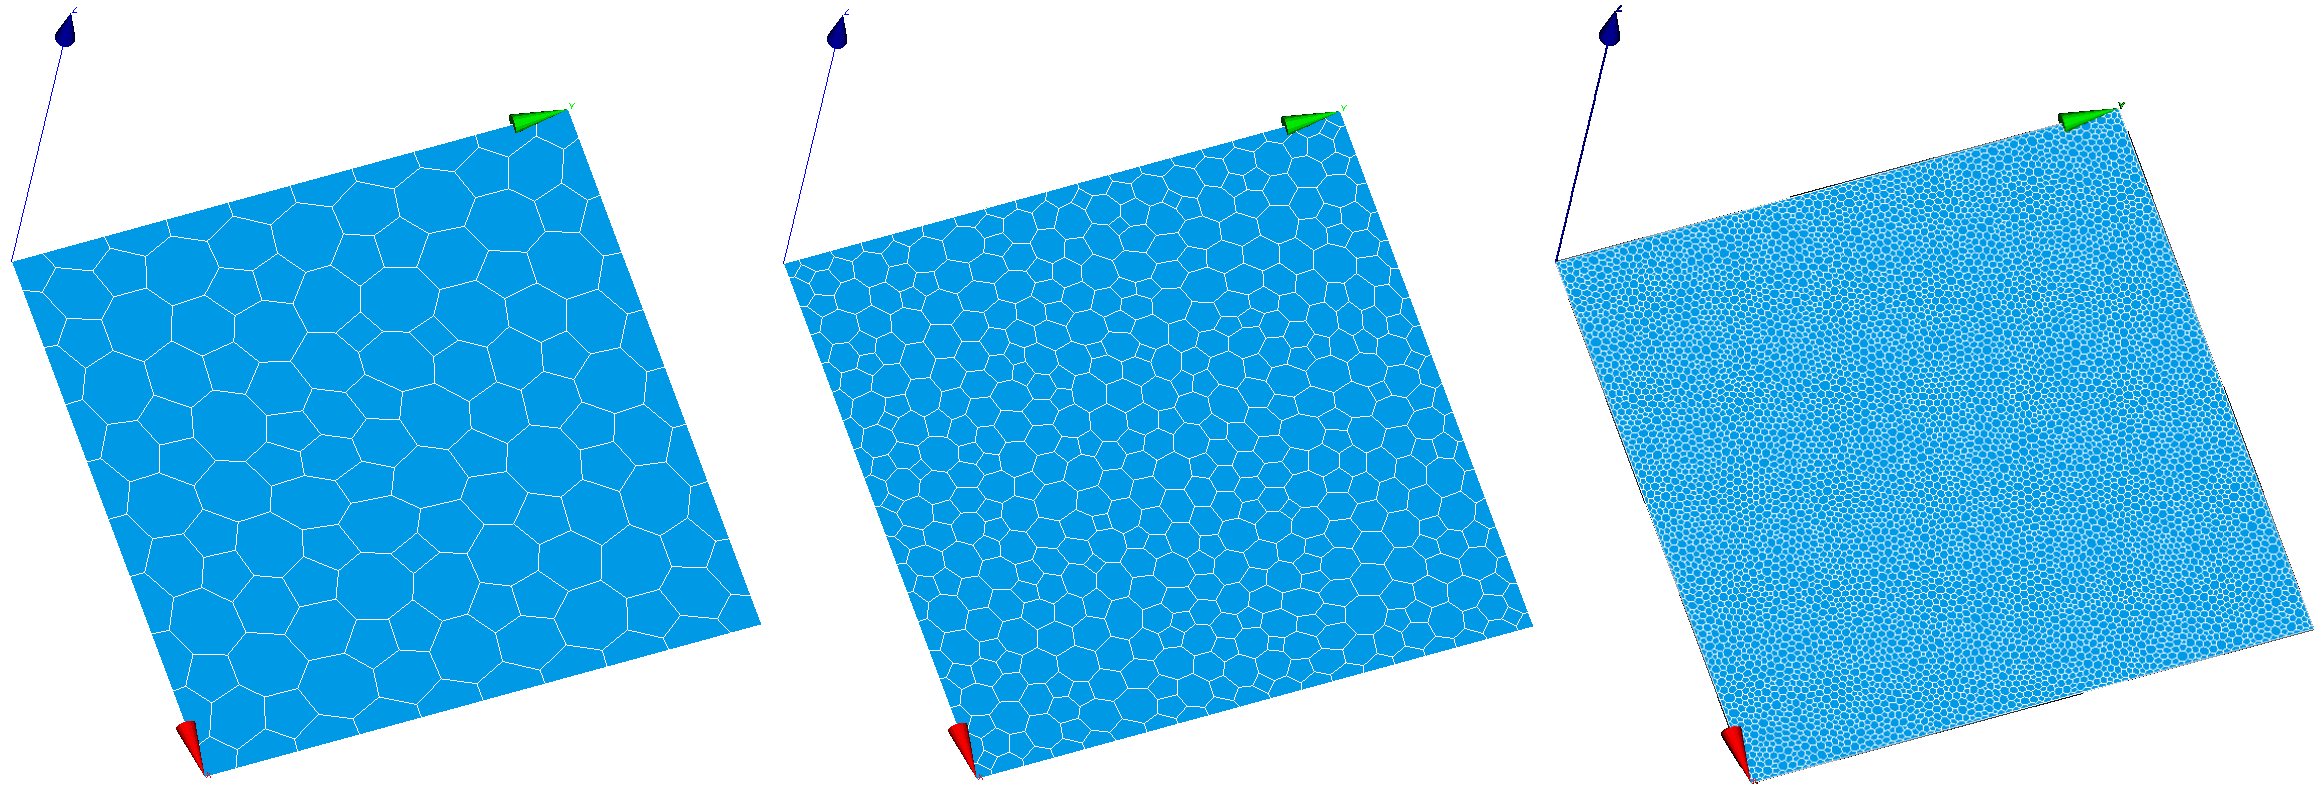
\includegraphics[width=1.0\textwidth]{./Images/polyMesh}
	\caption{\label{fig:polyMesh} Polygonal meshes generated with the ``smooth-dual'' approach. Refined from 135 to 6958 cells. Made with PDMT~\cite{Badri_pdmt}}
\end{figure}

\subsubsection{Numerical experiment}

We will use the Poisson equation as a model problem when we demonstrate how to set boundary conditions for an imported mesh that includes boundary indicators. The Poisson equation is the canonical elliptic partial differential equation. For a domain $\Omega \subset \mathbb{R}^2$ with boundary $\partial \Omega = \cup_{i = 0}^3 \Gamma_{D, i}$. For this numerical experiment we define the domain $\Omega$ by $[0, 2\pi] \times [0, 2\pi]$. As it seemed convenient for the test functions we are planning on using with the manufactured solution method.

\paragraph{Poisson's equation}
For this we decided to solve Poisson's Equation for a steady-state head distribution problem given by~:

\[
\boxed{\alpha~\Delta u(x,y) = - f(x,y) ~~~~\forall (x,y) \in \Omega},
\]\\
where~$\alpha = 1$~,~$f$ is a source term and $\Delta$ the Laplacian operator defined by~:
\[
\Delta{u(x,y)} = \frac{{\partial^2 u}}{\partial x^2} + \frac{{\partial^2 u}}{\partial y^2}.
\]

\paragraph{Boundary conditions}
As Poisson's equation is a boundary value problem we need to set boundary conditions to $\partial\Omega$. After multiple experiments, the best set that we ended up with was setting a Dirichlet conditions to the top and bottom edges of $\Omega^h$ and a Neumann condition to the left and right edges. Define for Dirichlet condition by~:
\[
u(x,y) = u_D(x,y)~~~~\forall (x,y) \in \partial\Omega_D,
\]
where, $\partial\Omega_D$ is the Dirichlet boundary of the domain $\Omega$ and $u_D(x,y)$ is the known value for $u(x,y)$. And for Neumann boundary condition~:
\[
\nabla u(x,y) \cdot n = u_N(x,y)~~~~\forall (x,y) \in \partial\Omega_N,
\]\\
where $n$ is the normal vector, and $u_N$ is the given Neumann condition on the border $\partial\Omega_N$

\paragraph{Manufactured solution}
Using the manufactured solution method, we first try to solve Poisson's with the test function~:
\[
u_m(x,y) = \cos(x)\sin(y)~~~~\forall (x,y) \in \Omega^h.
\]
To solve this equation with a numerical method we require source term $f_m$ and manufactured boundary conditions. To compute the manufactured source term,
\[
- f_m(x,y) = \frac{{\partial^2 u_m}}{\partial x^2} + \frac{{\partial^2 u_m}}{\partial y^2}.
\]
and with
\[
\frac{{\partial^2 u_m}}{\partial x^2} = -\cos(x)\sin(y)~\text{and}~\frac{{\partial^2 u_m}}{\partial y^2} = -\sin(y)\cos(x)
\]
we end up with \\
\[
\boxed{f_m(x,y) = 2\cos(x)\sin(y)}.
\]
\\\\
So that we end up with~:
\[
\boxed{\begin{cases}
	u(x,y)_{{\partial\Omega}_{top}^h} = \cos(x)*\sin(y) \\
	u(x,y)_{{\partial\Omega}_{bottom}^h} = \cos(x)*\sin(y) \\
	u(x,y)_{{\partial\Omega}_{left}^h} = \frac{\partial u_m(x,y)}{\partial n_1} = \sin(x)\sin(y) \\
	u(x,y)_{{\partial\Omega}_{right}^h} = \frac{\partial u_m(x,y)}{\partial n_2} = -\sin(x)\sin(y)
\end{cases}}
\]\\


\paragraph{TRUST~\cite{CEA_TRUST} and the ``PolyMac method''}

For the method, we decided to use a method currently under research at CEA called ``PolyMac'' that is currently implemented to the TRUST platform and is a form of Finite Volume Method. ``PolyMac'' has know several iterations since the past year and is starting to show promising results for some polytopal mesh simulation. While the method is still evolving, it is known to be close from the work in~\cite{bonelle2018new} and the ``Compatible Discrete Operator'', known as ``CDO'', method. Choosing the right method not being the goal for this phase, we did took an available method on a code we are used to work with and close to the development team to interface with our bench. Taking this as kind of a ``black-box'' simulation block in the pipeline. As we will explain later, the choice of the method and the physics we want to simulate is one of the main topics of our upcoming work. Thus, as nothing is set for now and we will likely change for other ones (e.g Discontinuous Galerkin (DG), Virtual Element Method (VEM)). We will then have to also search for the right implementation and code of such a method for our simulations.

\paragraph{Post-processing and error norms}

After getting our results from TRUST for all mesh types, we want to have a look at the convergence curves of the results along the refinements. To that end we will compute the $L_1, L_2$ and $L_\infty$ norms defined by

\[
L_1 = \int_{\Omega^h} \frac{|(u - u_m)|}{dA}
\]
\[
L_2 = \frac{\sqrt{\int_{\Omega^h}{(u - u_m)}^2}}{\int_{\Omega^h}dA}
\]
\[
L_{\infty} = \max{(\int_{\Omega^h} \frac{|(u - u_m)|}{dA})}~over~\Omega
\]\\
And will plot them in regards to the number of elements and the size f them in the meshes.

\subsubsection{Tools and pipeline}

To establish our benchmark, we utilized tools developed at CEA.~The SALOME platform~\cite{CEA_SALOME}, an open-source numerical simulation environment, supports CAD, meshing, and a variety of post-processing operations. However, to create a flexible and easily parameterized benchmark, we leveraged the extensive Python APIs available for interacting with SALOME.~We began by generating the geometry using the native SHAPER plugin, and then employed the GMSH~\cite{Geuzaine2009Gmsh} tool, integrated within SALOME, to create triangular and quadrangular meshes. These meshes were subsequently refined, as detailed in~\cref{refinements}.

\begin{figure}[htbp]
	\centering
	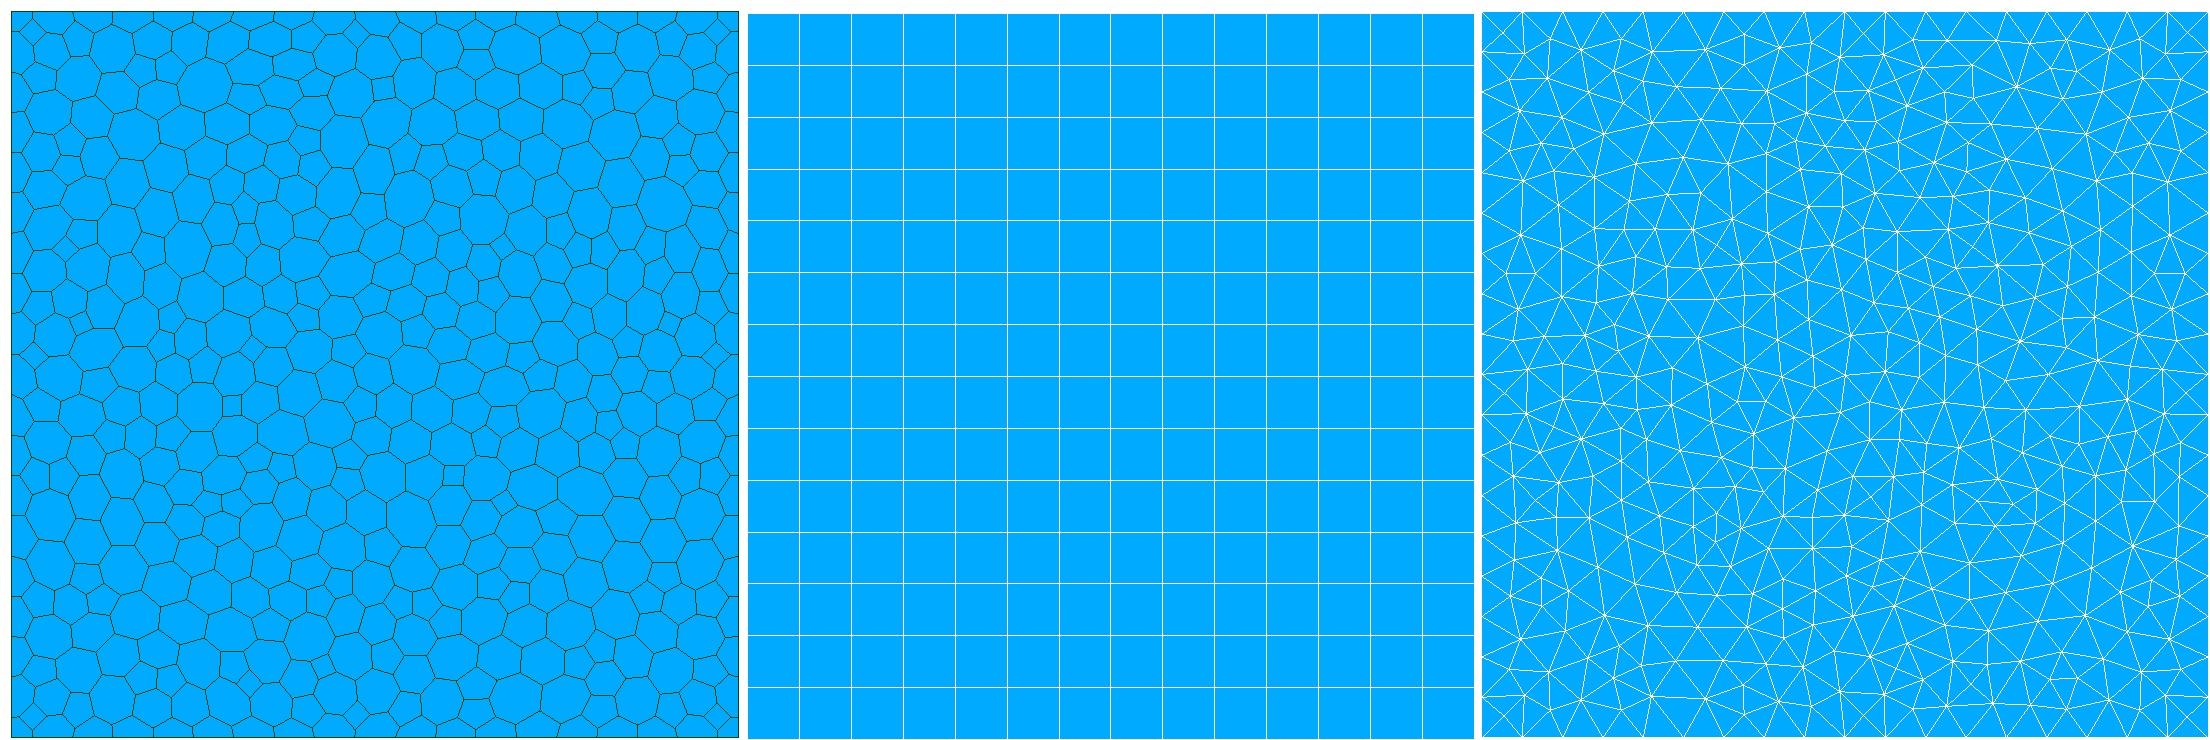
\includegraphics[width=0.8\textwidth]{./Images/refinements.png}
	\caption{\label{refinements} Polygonal, Triangular, Quadrangular and Triangular mesh on the $2\pi$ square. Generated with GMSH and PDMT mesher}
\end{figure}

After refining our meshes using the HOMARD module in SALOME, we sent the simulation to TRUST via Python, incorporating the meshes, simulation parameters, and pre-computed boundary conditions. With the simulation results from TRUST using PolyMac method, we post-process using Paraview. We recreated the exact solution provided by TRUST alongside the manufactured solution expected by $u_D(x,y)$ over $\Omega$. This allowed us to compute the difference $(u - u_m)$ which is necessary to evaluate the $L_1, L_2$ and $L_\infty$ norms for a given simulation. This process was repeated across all five refinements for the three types of meshes, and the resulting values were plotted. Additional python post-processing was carried out to calculate the order of convergence of these curves and to gather information about the meshes.

\subsubsection{Results}
In Paraview we then can se how the solution is distributed on $\Omega$ or even the error as in~\cref{polyPipeline}
\begin{figure}[htbp]
	\centering
	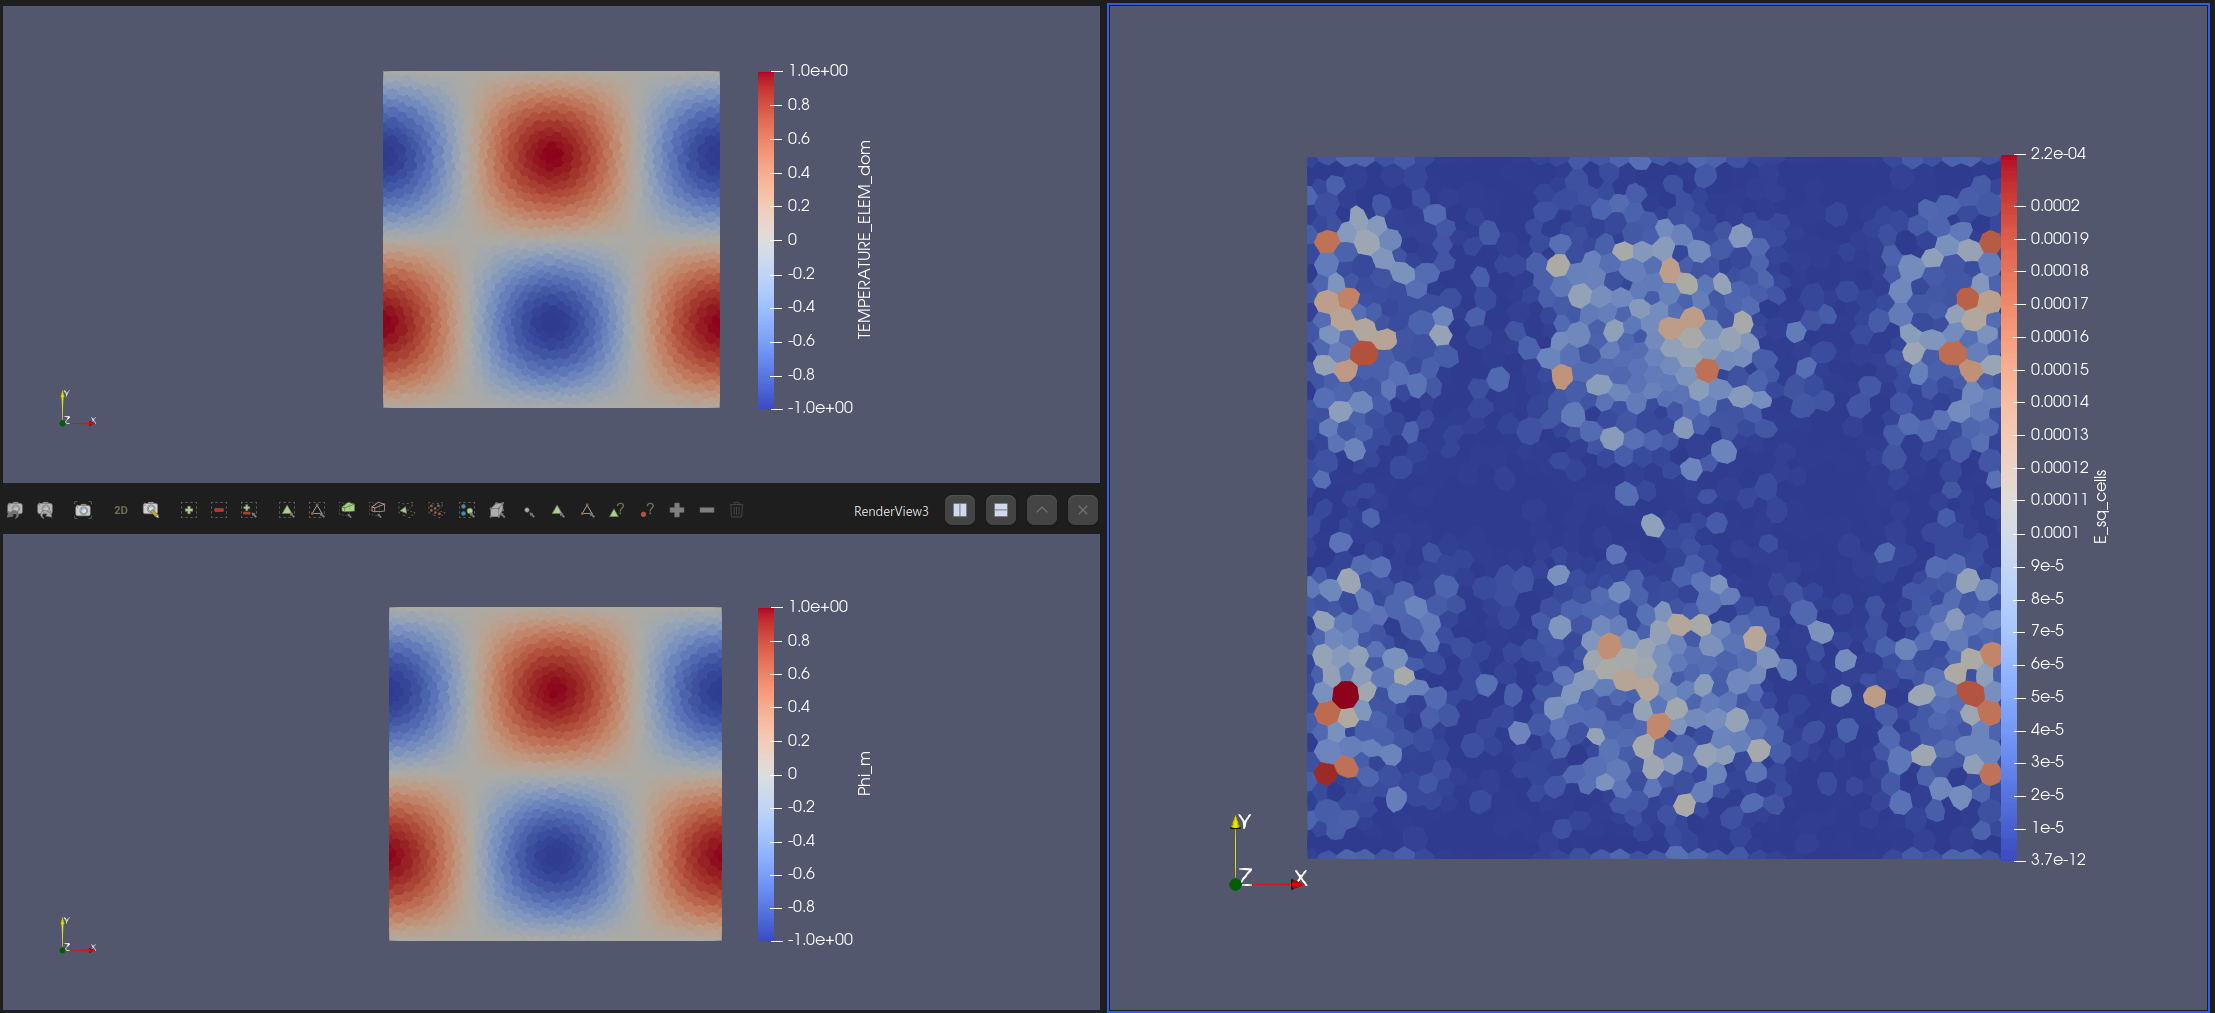
\includegraphics[width=1.0\textwidth]{./Images/polyPipeline.png}
	\caption{\label{polyPipeline} TRUST solution, Manufactured solution and L2 error over $\Omega$ for a 1783 polygon mesh}
\end{figure}
And compare those over different meshes and mesh types, c.f \cref{comTRI_POLY}
\begin{figure}[htbp]
	\centering
	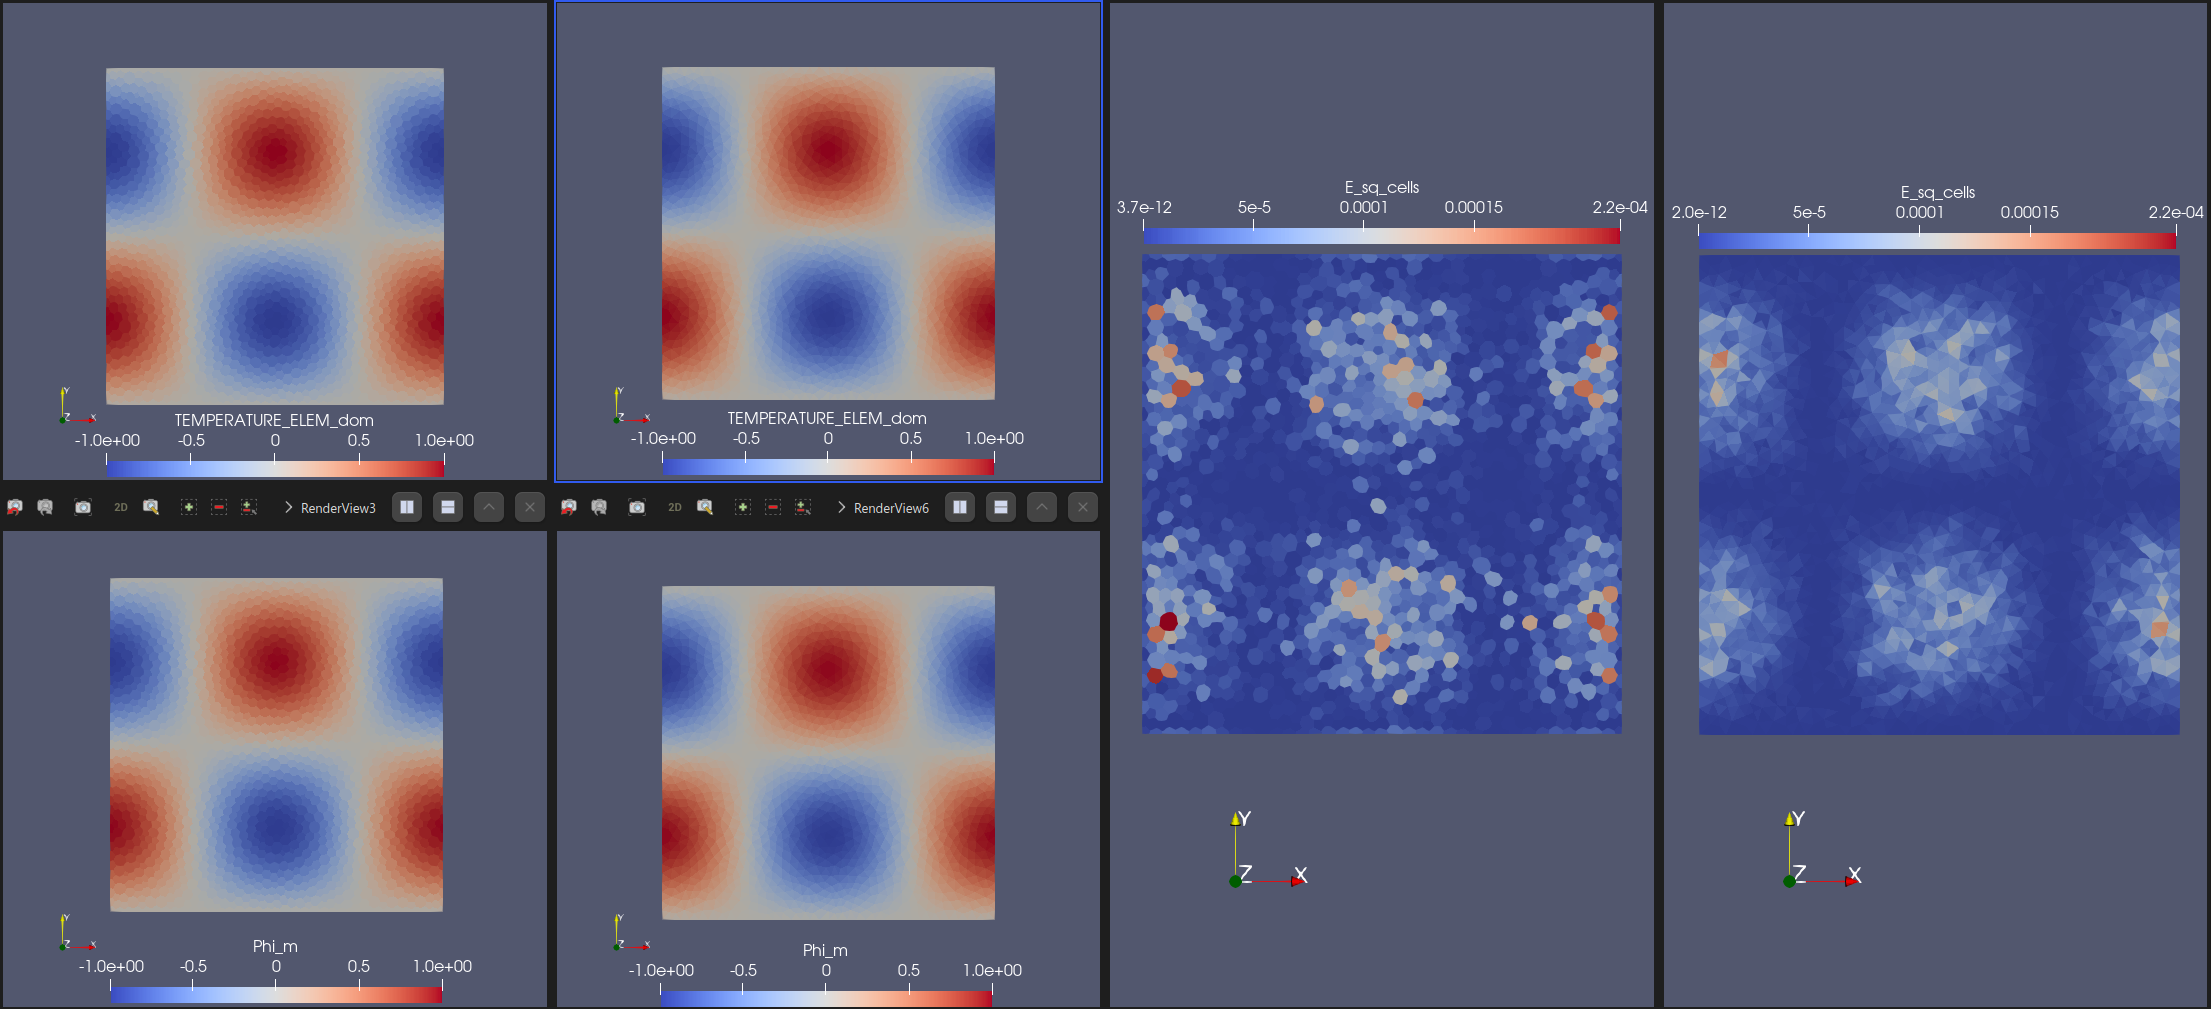
\includegraphics[width=1.0\textwidth]{./Images/comTRI_POLY.png}
	\caption{\label{comTRI_POLY} Comparisons following the same pipeline between triangular and polygonal meshes}
\end{figure}


Agglomerating those results then yield the following results detailed in \cref{ResultsBench} with the numbers of cells contained in the following table\\
\begin{center}
	\begin{tabular}{||c c c c||}
		\hline
		Refinement & Triangles & Quadrangles & Polygons \\ [0.5ex]
		\hline\hline
		1 & 232 & 49 & 135 \\
		\hline
		2 & 864 & 196 & 469 \\
		\hline
		3 & \color{red}3420 & 784 & 1783 \\
		\hline
		4 & 7634 & 1764 & \color{red}3926 \\
		\hline
		5 & 13626 & \color{red}3136 & 6958 \\ [1ex]
		\hline
	\end{tabular}
\end{center}

\begin{figure}[htbp]
	\centering
	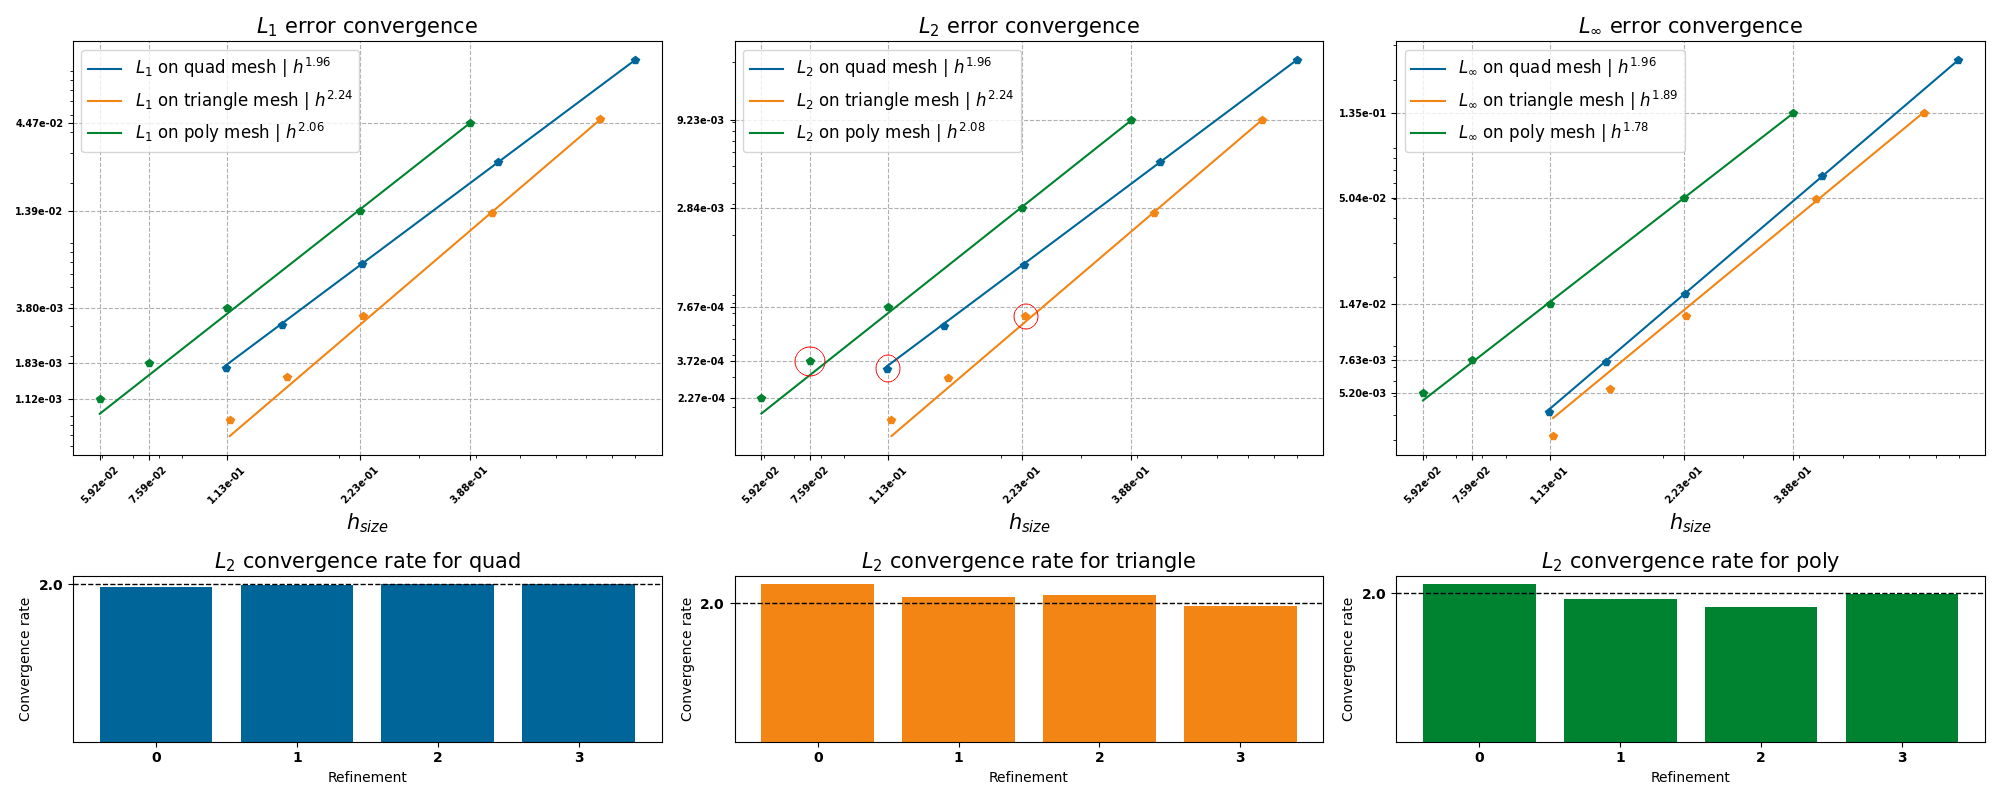
\includegraphics[width=1.0\textwidth]{./Images/ResultsBench.png}
	\caption{\label{ResultsBench} Comparisons following the same pipeline between triangular and polygonal meshes}
\end{figure}
The initial observation is that all models converge at a rate close to the expected $h^2$. Although the triangle and quadrangle meshes exhibit slightly lower error values compared to the polygonal meshes, this perspective shifts when considering the number of cells. For example, when comparing the three meshes with roughly the same number of elements (~3000+), the polygonal mesh shows a lower error than the triangular mesh. This observation aligns with similar findings in the community; however, expanding our benchmarking capabilities and increasing the complexity of the tests will be essential for further insights.

Our primary objective was to develop a flexible benchmark to evolve with ongoing studies and improve polytopal mesh simulations. We now have a fully automated, open-source Python code that generates, simulates, and post-processes multiple simulations. Moving forward, we aim to continually enhance this tool to make our benchmark more capable and robust as the complexity of our numerical simulations increases and we test a wider range of methods.

\section{Building upon those results}
After analyzing these preliminary results, we can reflect on how they were influenced by the entire process we selected, how they would hold up in a more realistic simulation framework, and how we can build upon them to develop our strategy for simulating with polyhedral meshes. The comparisons on how refinement impacted the error margin were conducted using a simple test function for a manufactured solution on a basic 2D geometry. Each of these input data points should now be challenged to assess how our results perform under different setups. Based on these subsequent results, we should be able to refine our strategy and ultimately reach a conclusion, allowing us to ``make an informed decision on how we intend to simulate polygonal and polyhedral meshes for adaptive mesh refinement''.

\subsection{How does those results scale with dimension and complexity?}
Going from 2D to 3D space could mean a lot to some simulation method or optimizations. Even still something yet to theorize in some case. For example, the dual approach used by PDMT to generate the polygonal meshes targeted by our benchmark cannot, as of today, generate a 3D mesh. So even if this technique has known asset for the adaptive mesh refinement part, we have no way to reproduce our benchmark study in 3D with this tool. Thus we have no way to see if the observed tendency to obtain roughly the same error as other mesh type but with a lower number of cells will translate in 3D.

\subsubsection{Geogram and Centroïdal Voronoi Tesselation}
Given this limitation, we had to explore alternative methods for meshing with polygons and polyhedral to properly validate our approach. Regarding polygonal/polyhedral mesh generation, we began investigating the potential of Centroïdal Voronoi Tesselation (CVT). In particular, we utilized the tool developed by Bruno Levy: Geogram [<insert ref>]. Geogram is a comprehensive library offering various tools to generate, visualize, modify, and clean a wide range of polygonal and polyhedral meshes. Following the initial benchmark results, we focused on generating similar polygonal meshes with comparable refinement levels to those previously used. Our objective was to replicate the benchmark setup and assess whether the obtained results would hold with CVT-generated polygonal meshes before applying this method to polyhedral meshes.

In parallel, Geogram's Vorpalite tool [<insert ref>] enabled us to generate polyhedral meshes using the same CVT technique. Building upon a plugin developed for the Salome platform [<insert ref>], we are also working on obtaining the first simulations using the PolyMac method on a 3D-square mesh. Since the simulation of tetrahedral and hexahedral meshes in 3D does not require such preparatory work, achieving this initial simulation with a CVT-generated mesh using TRUST and the PolyMac method will provide all the necessary components to recreate our benchmark study in 3D. As the focus of this research is on improving adaptive mesh refinement techniques for polyhedral meshes, we aim to confirm the trends observed in our results with these meshes.

We will further explore how CVT mesh generation could also provide a promising direction for the mesh refinement aspect of this research. As CVT generates polyhedral meshes with overall good quality and favorable properties, based on a set of points that can be positioned almost arbitrarily in space.

\subsubsection{Complexity of the solution}
As outlined in the benchmarking process, we have so far only used a very simple test function for our manufactured solution approach. Combined with the simple geometry, this means that we have not yet fully tested the limits of the method or examined its sensitivity to more complex test cases. Consequently, it remains unclear if and how these aspects might influence our results. To address this, we plan to extend our testing by applying the current 2D benchmark, as well as the upcoming 3D benchmark, to more complex test functions that are known for assessing the accuracy of simulation outcomes. We will progressively test more challenging functions until we are confident in the robustness of our solution. One of the first candidates for this is the Rastrigin function that, for \(n\) variables, is given by:
\[
f(\mathbf{x}) = A \cdot n + \sum_{i=1}^{n} \left( x_i^2 - A \cdot \cos(2 \pi x_i) \right)
\]
where:
\[
\mathbf{x} = (x_1, x_2, \dots, x_n)
\]
\[
A = 10
\]
\[
x_i \in [-5.12, 5.12]
\]

As it is a well-known non-convex mathematical function commonly used as a benchmark for evaluating optimization algorithms. It serves as a typical example of a multimodal function and has the added advantage of having a greater definition interval than our current [-\(\pi\), \(\pi\)] one. Beside that, as the TRUST teams is used to test their code using the FVCA Benchmark [] we are planning to also test our solution with this to compare the results obtained.
Following our exploration of the test function at the end of the pipeline, we will certainly examine the geometric aspect as well. However, since selecting an appropriate geometry may be intertwined with choosing the correct physics, we might need to make a decision on that before delving into this aspect.

\subsection{Do theses results translate to other methods, codes}
So far, we have only conducted simulations using the PolyMac method implemented in the TRUST code, as described in Section 2.2.2. However, as mentioned previously, numerous methods have emerged in recent years for performing simulations with polygonal and polyhedral meshes. This is closely linked to the physics we choose to simulate. Methods such as Discontinuous Galerkin (DG), Virtual Element Method (VEM), and Mimetic Finite Difference (MFD) have been the subject of extensive study in recent publications.

Exploring how we can simulate our test case using codes that implement these methods, and understanding the contributions they make to polyhedral mesh simulation, will be one of the next steps in assessing the behavior of these meshes. This will be a cornerstone in determining our strategy moving forward, as both the methods and the codes must align with our requirements for future research. They should effectively match the physics we wish to simulate, the geometry we intend to utilize, the adaptive mesh refinement (AMR) techniques we want to apply and explore, and must be robust and mature enough to build upon.

\section{Planned work}
The previous section addressed what we are currently undertaking and planning to pursue in the near future to expand upon our initial benchmark and its results. Here, we aim to outline our approach to achieving our goal of ``making an informed decision on how we intend to simulate polygonal and polyhedral meshes for adaptive mesh refinement'', as well as the avenues we plan to explore following the insights already presented.

\subsection{Formalizing our strategy for polyhedral numerical simulation}
The numerical simulation pipeline consists of several key steps, each requiring critical decisions tailored to the specific problem at hand. It can be divided into three main components: mesh generation, the simulation process, and the evaluation of results. Each stage involves a series of choices, which our study aims to guide.

\subsubsection{Meshing}
Although closely linked to the chosen physics for relevance, selecting an appropriate geometry is one of the key initial steps in the meshing process. Unlike hexahedral meshing, polyhedral meshing can be automated for any geometry. However, understanding the strengths and weaknesses of the meshing method we adopt will help us select geometries that either challenge or avoid potential edge cases. We have already explored two different meshing techniques for polygons that could be extended to polyhedrons: dual-meshing and CVT.\@ These methods take different approaches, and we are currently comparing them within our benchmarking framework. Our aim is to determine whether both methods are worth further investigation or if we can already make a definitive choice. While CVT can generate 3D polyhedral meshes, it still presents challenges with adaptive mesh refinement (AMR), whereas dual-meshing benefits from tetrahedral mesh AMR but currently lacks the capability to generate 3D meshes. Additionally, each meshing tool associated with a specific meshing method comes with its own set of inputs and tuning parameters. Understanding the underlying principles of these meshers will enable us to fine-tune our simulations and better anticipate their capabilities.

\subsubsection{Simulation}
The simulation block involves deciding what we want to simulate and how to simulate our test cases. This includes selecting the physics we aim to model, the numerical method to be used, and the code that implements that method. In recent research publications related to polyhedral meshes, certain fields of physics, such as magnetism, computational fluid dynamics (CFD) for high-speed flows, and elasticity problems, have emerged as particularly relevant. Focusing on physics that already tend to favor polyhedral meshes or benefit from them could amplify the impact of our work if we succeed in improving the simulations. Additionally, aligning our efforts with simulations that are similar to those conducted by research teams in these areas can not only support their findings but also provide us with new insights and directions for further work

Similar to the selection of physics, the methods used in recent publications on polyhedral mesh simulations appear to be converging. Methods such as Discontinuous Galerkin (DG), the Virtual Element Method (VEM), and Mimetic Finite Difference (MFD) have gained particular interest. PolyMac, which we have already employed for our benchmarking, also shows promise as a viable candidate. Each method, along with more traditional Finite Element Methods (FEM), presents specific advantages and drawbacks. However, as each physics community gravitates toward particular methods for their simulations, we should be able to select the most appropriate method based on the physics we choose to model. Additionally, we will need to evaluate the performance of each method in the context of adaptive mesh refinement and its behavior with higher-order accuracy.

\subsubsection{Evaluation}
Beyond selecting the appropriate method for simulating polytopal meshes, the evaluation of their performance is equally crucial. There are numerous error estimators available, along with various techniques for assessing mesh quality and the accuracy of the results. For now, we have decided to focus on the convergence of $L_1 , L_2$ and $L_{\infty}$ norms defined earlier. Depending on the physics we ultimately simulate and the estimators we utilize, we may need to adjust our post-processing pipeline accordingly.

Regarding polytopal simulations, another question arose during our tests that was briefly addressed in the methods section: how do we measure $h_{size}$ for a polytopal mesh? Although we have made a preliminary choice for these initial polygonal simulations, we recognize that we will need to carefully consider this aspect to provide a definitive answer, given the importance of this value in computing the convergence of the method on a mesh.

\subsection{Leads on improving adaptive mesh refinements}

After establishing our strategy for simulating polyhedral meshes, we can now outline the primary objective of this thesis: how to efficiently refine polytopal meshes? While some techniques are already functional, they predominantly rely on refining the same mesh or utilizing an underlying tetrahedral mesh.

\subsubsection{Existing AMR techniques for polytopal meshes}
For instance, tree-based approaches, such as those presented in~\cite{chau2018polytree}, yield results similar to those shown in~\cref{polytree}, but these methods are specifically designed to refine a single mesh. Although this approach may be applicable in certain scenarios and could be investigated during this thesis, our immediate focus is on a more dynamic remeshing strategy.

\begin{figure}[htbp]
\centering
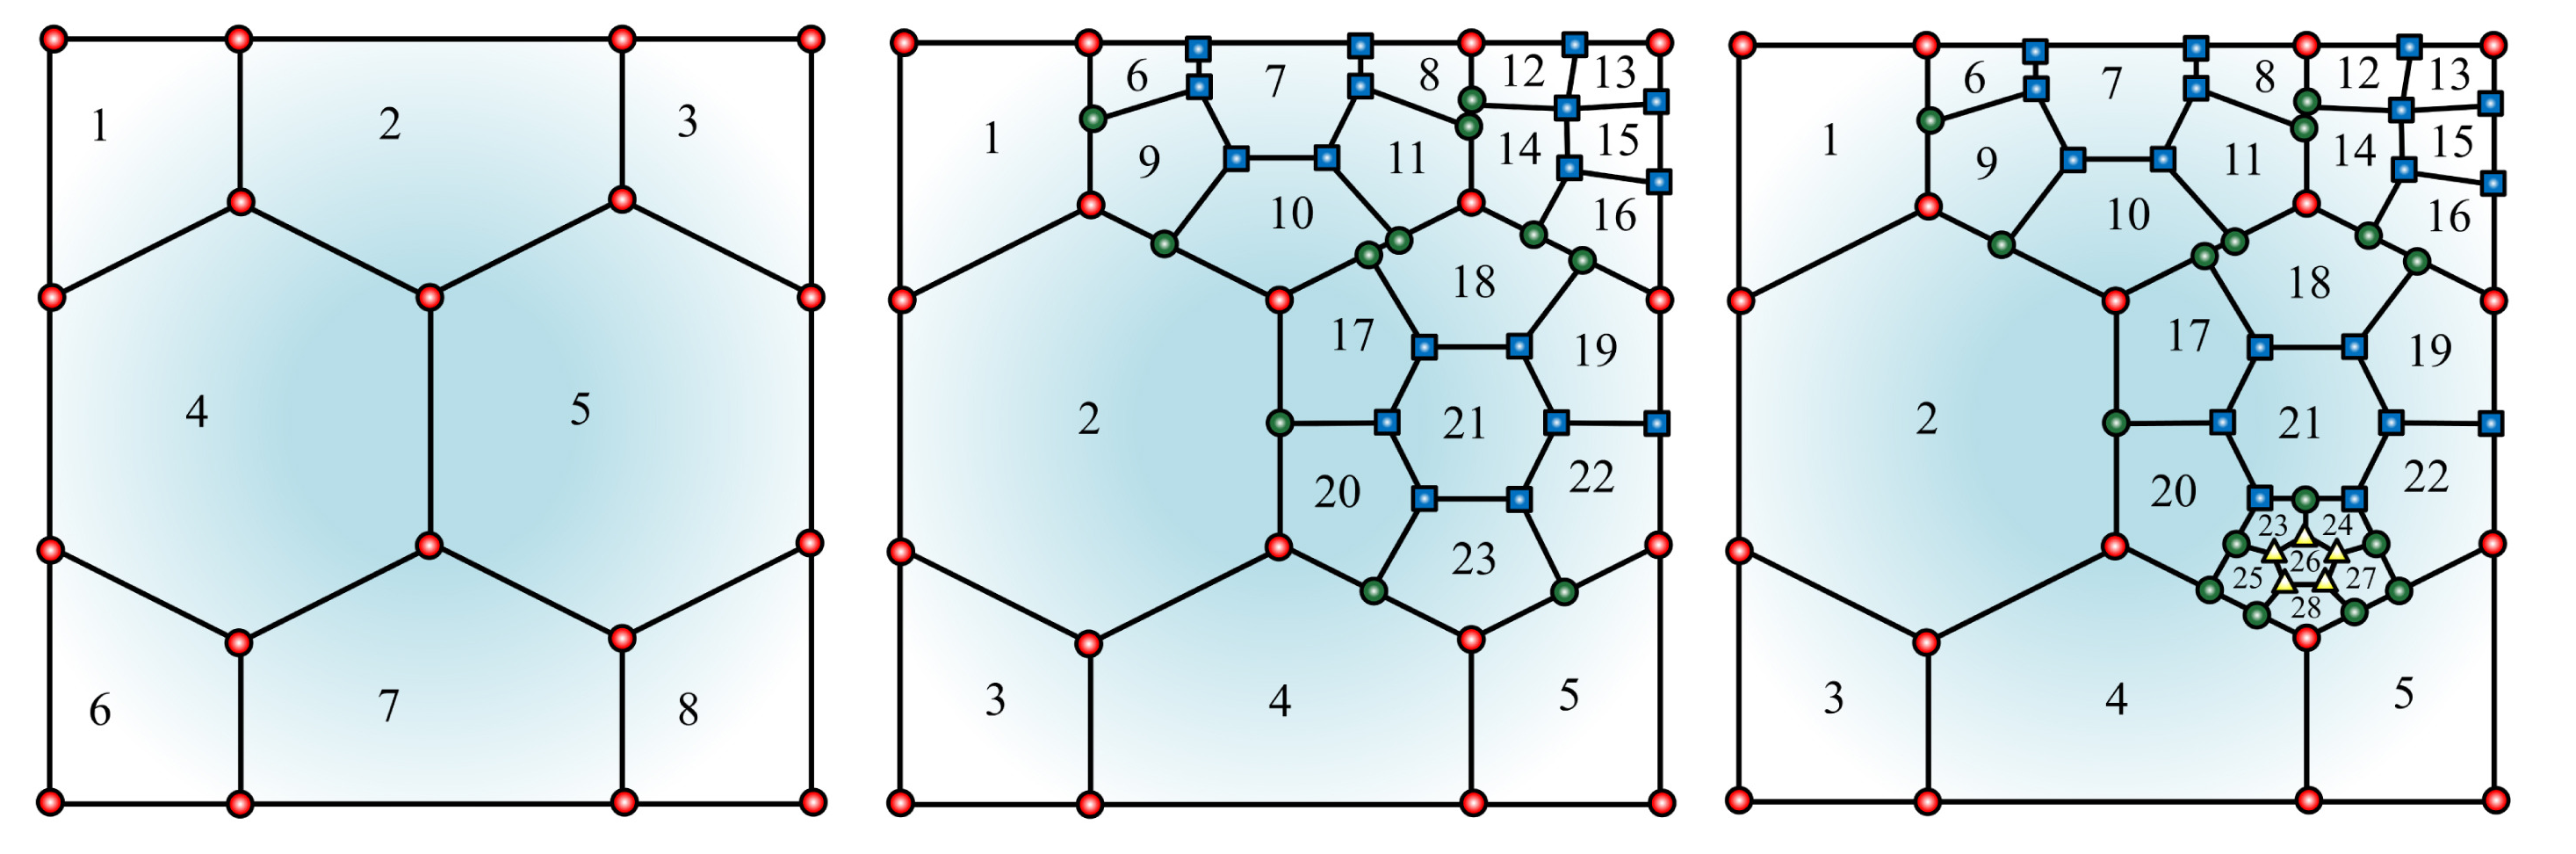
\includegraphics[width=0.7\textwidth]{./Images/polytree}
\caption{\label{polytree} A 3-level polytree meshes refinement from~\cite{chau2018polytree}.}
\end{figure}

Another promising method for adaptive mesh refinement in polyhedrons involves the “Dual” and “Smooth-Dual” approaches. These methods leverage an underlying triangular mesh, thereby benefiting from the established adaptive mesh refinement technologies developed for triangles and tetrahedra. However, a significant drawback of these methods is their current inability to produce 3D meshes. Nevertheless, a key focus of this thesis will be to explore the potential of using the “Smooth-Dual” approach to generate 3D meshes. The adaptive mesh refinement aspects of simulating these meshes will closely resemble those utilized with tetrahedrons. Results of refinement in 2D are illustrated in figure~\ref{fig:smoothDUAL}.


\begin{figure}[htbp]
\centering
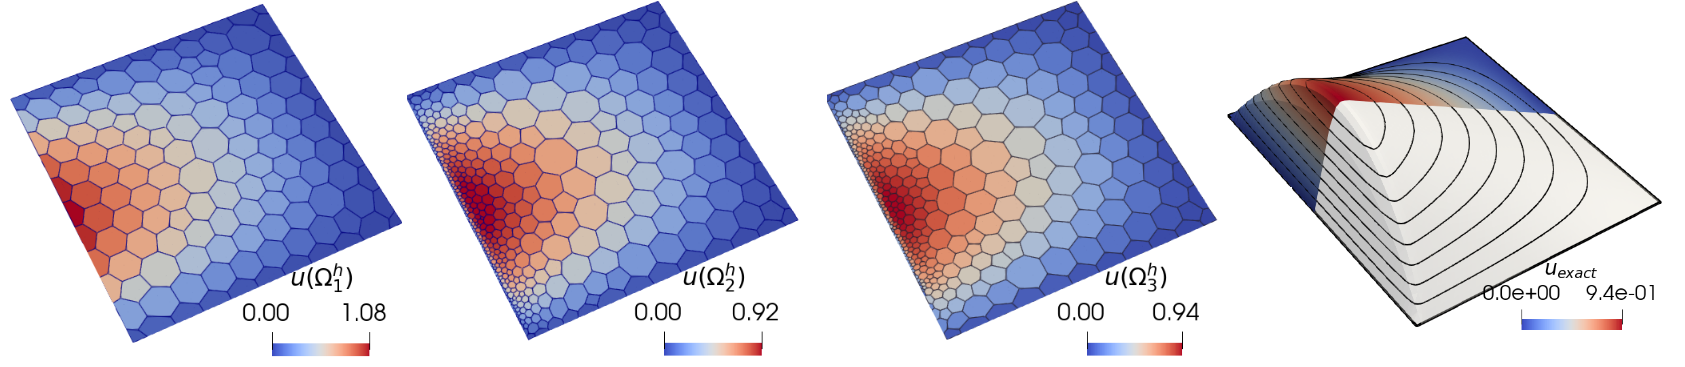
\includegraphics[width=1.0\textwidth]{./Images/smoothDUAL}
\caption{\label{fig:smoothDUAL} A polygonal mesh generated and refined with the Smooth-Dual approach.}
\end{figure}

\subsubsection{A CVT-base approche to AMR}
The third approach we are considering does not seems to have been explored yet as a method for adaptive mesh refinement. With the initiation of mesh generation using Centroïdal Voronoi Tesselation (CVT) we have our mesh $\Omega^h =  \bigcup\limits_{i=1}^{N_{\mathcal{P}}}  \mathcal{P}_i $, where $\left\{\mathcal{P} \right\}{_{i=1}^{N_{\mathcal{P}}}}$ is our set of $N_{\mathcal{P}}$ polygons or polyhedrons. Given that the CVT was seeded by ${N}_P$ points, we now have a density $\mathcal{D}({P}_i$) link to the tightness of the mesh. Knowing that those seed point also have a $\omega_{P_i}$ weight inside the CVT definition, we could explore finding a way to link $\mathcal{S}_i$ the seed set, those $\omega_{P_i}$ weights and the function we are simulating $u(\mathbf{x})$. This would create a loop between our numerical simulation results and a tailored CVT mesh generation to adapt the mesh by iterations. This is largely speculative at the time but as seen in~\cite{voroGPU} we can see promising results on a refined CVT-based polyhedral mesh on the figure~\ref{fig:voroGPU}

\begin{figure}[htbp]
\centering
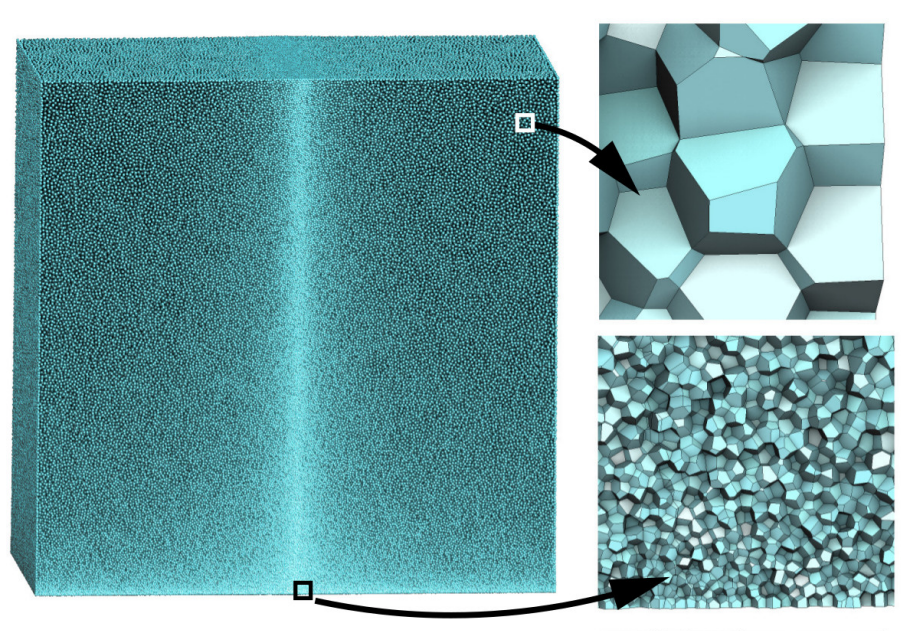
\includegraphics[width=0.7\textwidth]{./Images/voroGPU}
\caption{\label{fig:voroGPU} A point-set of 10 million points with varying density. With closeups on cross-sections of the Voronoi diagram. Image from~\cite{voroGPU}.}
\end{figure}

\section{Conclusion}

\bibliographystyle{ieeetr}
\bibliography{./biblio.bib}

\end{document}
